\chapter{Implementation}\label{Implementation}
\section{Architecture}
\subsection{Componenets}

To set up the network we need several physical devices. The physical devices used in this set up are:

\begin{enumerate}
    \item ASUS UX360 Laptop
    \item One Raspberry Pi 4 B 8Gb
    \item Two Raspberry Pi 4 B 4Gb 
\end{enumerate}

In addition to these devices a desktop PC is also used, but is not part of the network. The desktop is used to control all the other devices through SSH, and also contained a Linux virtual machine for building components in.


\subsection{Initial Setup of Machines}
Setting up the machines requires installation of the correct operating systems, software, source code, Paths and other configurations.

\begin{table}[htb]
    \caption{Software and Versions for Devices}
    \renewcommand{\arraystretch}{2}
    \begin{tabular}{|p{2cm}|p{2.5cm}|p{2cm}|p{2.2cm}|p{2.2cm}|}
      \hline
        \textbf{Device}         & \textbf{Operating System}    & \textbf{Docker}               & \textbf{Docker Compose} & \textbf{Go}         \\[10pt] \hline 
        \textbf{Laptop}         & Ubuntu 20.04LTS              & 19.03.12 - Community          &  1.26.2              & go1.15.5 linux/amd64   \\[10pt] \hline 
        \textbf{Raspberry Pi}   & Raspbian OS 64-bit (beta)    & 19.03.12 - Community          & 1.21.0               & go1.15.5 linux/arm64   \\[10pt] \hline 

    \end{tabular}
\end{table}

In addition to installing Go on each device using the standard installation and Path setting, a GOPATH must also be set
\begin{verbatim}
     $ export GOPATH=$HOME/go
     $ mkdir -p $GOPATH/src/github.com/Hyperledger
     $ git clone -b release-2.3 https://github.com/hyperledger/fabric.git
\end{verbatim} 

Hostnames and IP addresses of each device must also be recovered, using the following commands respectively
\begin{verbatim}
    $ hostname
    $ hostname -I
\end{verbatim}
If machines have duplicate hostnames, as occurs with Raspberry Pi's, then new hostnames must be set. The following command can help set a new hostname:
\begin{verbatim}
    $ sudo raspi-config
\end{verbatim}
From there navigate to network options, where hostname can be set. 


\subsection{Connecting Machines}

In order to connect the machines to allow the Hyperledger Fabric network to communicate all the devices must be joined in to a Docker Swarm. The following command should be run from the laptop that will be a part of the network.

\begin{verbatim}
    $ docker swarm init
\end{verbatim}
\begin{figure}[h]
    \centering
    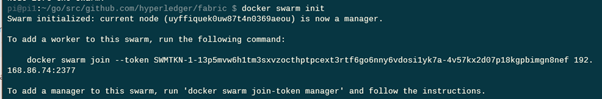
\includegraphics{images/docker swarm.png}
    \caption{Output of docker swarm init command}
    \label{fig:my_label}
\end{figure}

The resulting command should be copied and run in each device that will become part of the network.

Following all machines being a part of the swarm, a network overlay must be created, this is network layer where the machines where docker containers can communicate through. This is create through the following command, on a manager of the docker swarm.

\begin{verbatim}
    $ docker network create --attachable --driver overlay pi-network
\end{verbatim}

\begin{figure}[h]
    \centering
    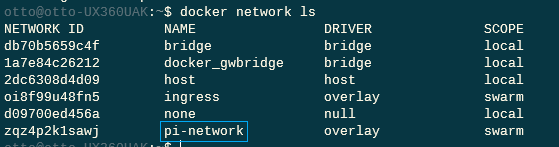
\includegraphics{images/networkoverlay.png}
    \caption{Result of creating a network overlay}
    \label{fig:my_label}
\end{figure}

\section{Making HLF arm64 compatible}


\subsection{Creating Binaries}

As Hyperledger expects a 64 bit operating system, the normal Raspberry Pi operating system will fail here, and the 64 bit OS must be used. 
In order to create the binaries that allow you to use the Hyperledger Fabric network, you must go into the source code directory of Hyperledger Fabric that was cloned before. 
Using the Makefile provided in the fabric repository, creating the binaries is quite simple, from inside one of the Raspberry Pis:
\begin{verbatim}
    $ cd $GOPATH/src/github.com/hyperledger/fabric
    $ make native
\end{verbatim}



The ARM64 binaries will be be in the build/bin folder of the repository and should be copied out to another folder for later. They have also been copied into the Github repository for this project in bin\_raspbian.


\subsection{Creating Docker Images}

Hyperledger provides Docker images on Dockerhub for people to use, however these images are like the binaries only x86-64 compatible, so we must make our own ARM64 compatible images.

This is achieved using Buildx, a new experimental feature that allows the building of images for multiple architectures at a time. 

For this project a Linux Mint virtual machine was created in Oracle VirtualBox on a desktop PC. Go will have to be installed and GOPATH set like in the other machines.

\begin{verbatim}
     $ export GOPATH=$HOME/go
     $ mkdir -p $GOPATH/src/github.com/Hyperledger
     $ git clone -b release-2.3 https://github.com/hyperledger/fabric.git
\end{verbatim} 


In order to use Buildx to make ARM64 images the following  files in the Fabric source code must be edited.
\begin{itemize}
    \item Makefile
    \item docker-env.mk
    \item images/orderer/Dockerfile
    \item images/peer/Dockerfile
    \item images/tools/Dockerfile
\end{itemize}

The changes to these files has been included in the appendices, and these files have been included in the project Github repository.

Using Buildx requires also setting up QEMU(QEMU is a virtualizer/emulator) and setting up some Buildx specifics:
\begin{verbatim}
    $ docker run --rm --privileged multiarch/qemu-user-static --reset -p yes
    $ docker buildx create --name mybuilder
    $ docker buildx use mybuilder
\end{verbatim}

Following this the images can be created, each image was created individually using the following commands:

\begin{verbatim}
    $ make baseos-docker
    $ make peer-docker
    $ make orderer-docker
    $ make ccenv-docker
    $ make tools-docker
\end{verbatim}

The process of creating these images can take a while, and the output will fail at the very end, as the Makefile will attempt to tag the docker images but as we have created images with names the Makefile was not expecting, however the image is created which can be viewed using:

\begin{verbatim}
    $ docker images
\end{verbatim}
\textit{The output of creating a peer using this method has been included in the appendices.
The images have also been pushed to the Dockerhub repository associated with this project, and can be pulled and used without going through this long and complicated process.
}
\section{Defining the Network}

Before a Hyperledger Fabric network can be started, alot of configuration files must be created that will define the network participants, policies and details on the network participants such as IP addresses and host machines. This section goes through the setup.

\subsection{Cryptographic Materials}

For this thesis, as the network is not a production network, as certificate authority is not used to generate and distribute cryptographic materials, instead the Cryptogen binary is used which creates all the necessary cryptographic materials which need to be copied to each device in the network. 

Cryptogen consumes a crypto-congfig.yaml file which contains the definitions of organisations in the network, the IP addresses ascociated with the organisations and type of the organisations.

\begin{figure}[H]
    \centering
    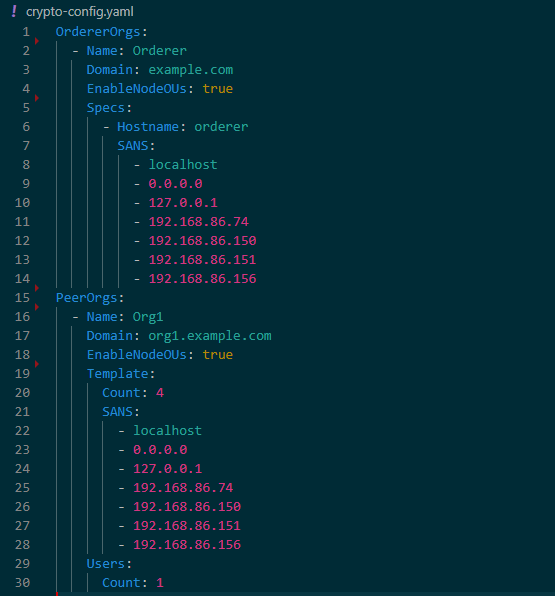
\includegraphics{images/cryptoconfigyaml.PNG}
    \caption{Contents of crypto-config.yaml}
    \label{fig:my_label}
\end{figure}

\begin{verbatim}
    $cryptogen generate --config=./crypto-config.yaml --output="organizations"
\end{verbatim}

This command generates the cryptographic material, creates an 'organizations' folder and places the generated material in it, this is the folder that must be shared to other devices.

\subsection{Channel Configuration}

For a network to start, it must be given a genesis block from which nodes in the network can access the policies and organisations on the network, this is created in this step.

Hyperledger Fabric makes use of a binary called \textbf{configtxgen} that consumes a configtx.yaml file. This configtx file contains organizations, capabilities, application, orderer, channel and profile sections.


\begin{itemize}
    \item[\textbf{Organizations}]
        
        This section defines the different organisations that are part of the channel, containing organisation specific policies, MSP configuration paths and orderer endpoints.
    \item[\textbf{Capabilites}]
        
        This defines the capabilties of the channel, refering to the different versions of Hyperledger Fabric, this project uses version 2 capabilities.
    \item[\textbf{Application}]
    
        This section defines the values to encode into a config transaction or genesis block for application related parameters
        
    \item[\textbf{Orderer}]
    
        This section defines the concensus type, of the channel, which in this case uses Raft, referred to as EtcdRaft in Hyperledger.  It also details consensus policies such as size of blocks. It also contains consensus policies.
    \item[\textbf{Channel}]
    
        Defines channel policies such as how many admin users are required to change a channel policy.
    \item[\textbf{Profile}]
    
        This sections allows for diferrent configuration profiles to be created into one configtx.yaml file, in the case of this project, only one profile is set and follows defaults.
\end{itemize}

\textit{The configtx.yaml file used in this project is included in the Github repository}

Once the configtx.yaml file has been created and customised for the project, the block can be created with the \textbf{configtxgen} binary as follows:
\begin{verbatim}
    $ configtxgen -profile TwoOrgsApplicationGenesis -outputBlock
    ./channel-artifacts/pichannel.block -channelID pichannel
\end{verbatim}
\begin{figure}[h]
    \centering
    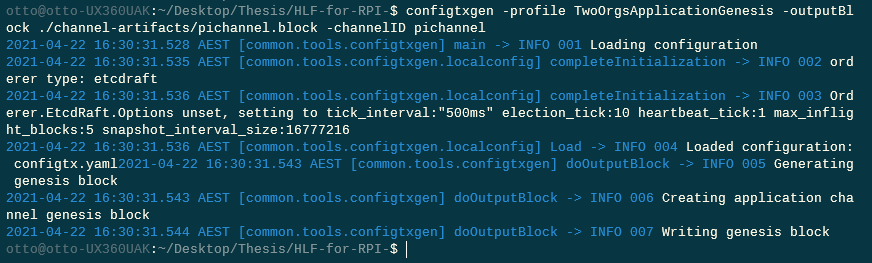
\includegraphics[width=1.2\columnwidth]{configtxgen.PNG}
    \caption{Output from configtxgen binary}
    \label{fig:my_label}
\end{figure}

\subsection{Configuring Peer and Orderer Nodes}

When creating a peer node, the peer expects to have access to a core.yaml file, which contains all the configurations of the peer. In a similar way the orderer node expects a orderer.yaml file. However the Peer and Orderer docker image contains with them these files that contains all the default settings for the node, many of which do not need to be changed.

All of these defaults can be overwritten in another yaml file which is used to create the containers from the Docker images. The following images show how to change a core.yaml variable into an environment variable.

\begin{figure}
    \centering
    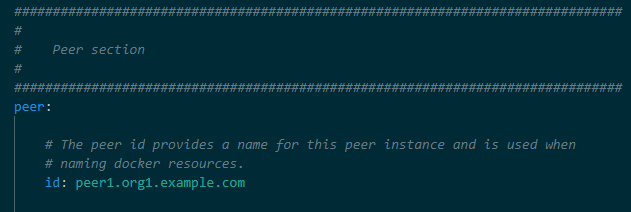
\includegraphics[width=\textwidth]{peercoreyaml.PNG}
    \caption{Variable in core.yaml}
    \label{fig:my_label}
\end{figure}

\begin{figure}
    \centering
    
\includegraphics[width=\textwidth]{peer envirovar.PNG}
    \caption{Same variable, using an override in environment variables}
    \label{fig:my_label}
\end{figure}

\subsubsection{Peer Configuration}

For this project the variables shown in this image are the ones we set ourselves. For each different peer a new Peer ID must be set, that is unique in the network, the addresses may use the Peer IDs used in the network as docker containers can use these IDs to resolve addresses. Ports must also configured, as each peer uses multiple ports for connecting with other peers, connecting with their chaincode containers and for exposing themselves for monitoring.



\begin{figure}[h]
    \centering
    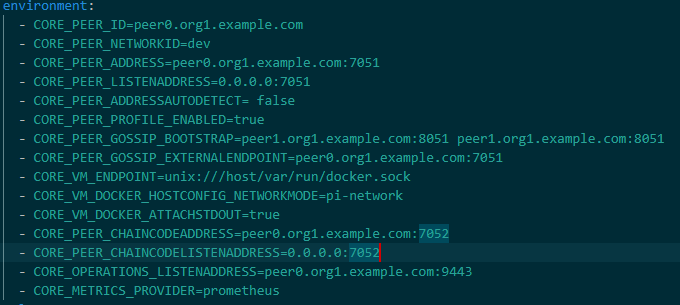
\includegraphics[width=1\columnwidth]{peer enviro.PNG}
    \caption{Example of the Peer variables we must control}
    \label{fig:my_label}
\end{figure}


\subsubsection{Ordering Configuration}

Setting an Orderers variables is very similar to a Peers variables, the main distinction is that Orderer Admin certificates must be provided. This is a new feature of Hyperledger Fabric version 2.3, where Orderers are now responsible for the creation of a channel, and as such now require admin certificates. 


A full explanation of each of these variables is provided in the Hyperledger Fabric source code within their core.yaml and orderer.yaml files.


\begin{figure}[h]
    \centering
    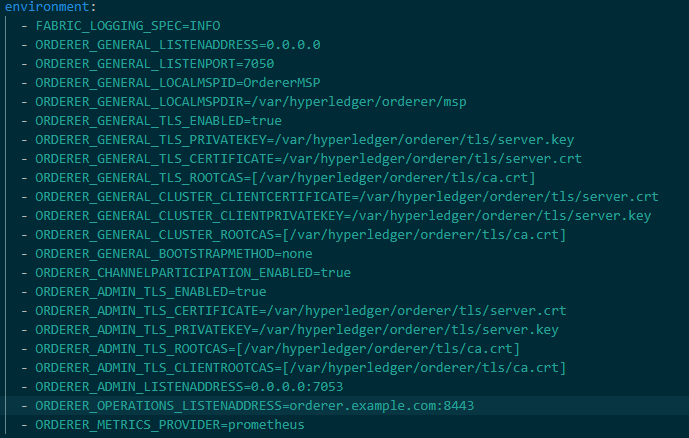
\includegraphics[width=1\columnwidth]{ordererenviro.PNG}
    \caption{Example of the Orderer variables we must control}
    \label{fig:my_label}
\end{figure}

\subsection{Docker Stack File}

All of these peer and orderer configurations must be set for each node that is to be part of the network. To allow for the network to be easily created on one machine and the containers to be spun up on the other machines across the network, a Docker Stack may be used, the Hyperledger test network only uses Docker Compose which is limited to only working on one machine. 

To use Docker Stack, a Docker Stack file must be created that has been called pi-network.yaml.
This file must be set to version 3, and each container must be described as a service. When defining a service, several fields must be set.
\begin{enumerate}
    \itemsep0em
    \item \textbf{Image} \\
        This is the image a container will use when it starts up, in this thesis it is important that all nodes destined to be on Pi's use the arm64-2.3 tagged images.
    \item \textbf{Environment} \\
        This is where the core.yaml file values are over written as demonstrated earlier
    \item \textbf{Volumes} \\
        Giving a service volumes means that when they start, provided a way to store cryptographic material and other necessary files and also for storing data that they create.
    \item \textbf{Working\_dir} \\
        This gives the containers of the service the location of where they should be working in the container.
    \item \textbf{Command} \\
        This is the command that service uses to start up the container it is to create.
    \item \textbf{Ports} \\ 
        These define the mapping from the host machines port to the containers ports
    \item \textbf{Hostname} \\
        This gives the service a name that the host machine is able to view, to interact with the containers created.
    \item \textbf{Networks} \\ 
        This define which network the service will be apart of, within networks a alias is also set that allows other containers on the network to communicate to.
    \item \textbf{Deploy} \\ 
        This defines the placement of the container created by the service in the swarm, it allows us to set a specific container to appear on a specific device, allowing us to place our arm64 based containers on the Raspberry Pi's. This should be equal to the hostname of the machine the service is destined to be placed on, found earlier using the \texit{hostname} command.
\end{enumerate}

\textit{This file is included in the Github repository and a collapsed version has been included in the appendices. }

\section{Starting the Network}

Once all configuration material, the docker images and binaries have been created they must be placed on the devices. 

All of the created material has been pushed into a Github repository which has then been cloned onto every machine. This ensures that all cryptographic material is the same across all devices, it also ensures that devices have access to the binaries they need to acces. Inorder to get the x86-64 binaries required by the Asus laptop, they were copied from the Fabric Samples repository. In addition to copying the binaries, Fabric Samples also contains already created chaincode applications, these also copied into the Github repository, to allow for testing if the Raspberry Pi's could also run chaincode as a part of the network.

As the Docker Images were pushed to Dockerhub, the images can be easily pulled down to the Raspberry Pis, bash scripts have been included in the Github repository which can be used to pull the correct images into the Raspberry Pi's and the Laptop.
The binaries must also be added to the \$PATH of each device, the following commands allow for this, and should be run from within the cloned git repository
On the Pis this command should be run(permissions may also need to be granted):
\begin{verbatim}
    chmod +x pull-hlf-arm-images
    sh pull-hlf-arm-images.sh
    cd bin_raspbian
    export PATH=${PWD}:$PATH
    cd ..
\end{verbatim}
On the Laptop this command should be run:
\begin{verbatim}
    chmod +x pull-hlf-arm-images
    sh pull-linux-images.sh
    cd bin_linux
    export PATH=${PWD}:$PATH
    cd ..
\end{verbatim}


\begin{table}[h]
\caption{Devices Information}
\begin{tabular}{|p{3cm}|p{3cm}|p{3cm}|p{3cm}|}
\hline
Device & Hostname      & IP Address     & HLF Node \\ [10pt] \hline
Laptop & otto-UX360UAK & 192.168.86.156 & Peer0    \\ [10pt] \hline
Pi1    & pi1           & 192.168.86.74  & Peer1    \\ [10pt] \hline
Pi2    & pi2           & 192.168.86.151 & Peer2    \\ [10pt] \hline
Pi3    & pi3           & 192.168.86.150 & Orderer  \\ [10pt] \hline
\end{tabular}
\end{table}


\subsection{Docker Stack Deploy}

All setup work for the network should now be done and deploying the stack can occur. Deployign the stack is as simple as the command below once everything else has been set up. The following command can be run from any device on the network, but in this case has been run from the Laptop.

\begin{verbatim}
    docker stack deploy --compose-file pi-network.yaml PiStack
\end{verbatim}

\begin{figure}
    \centering
    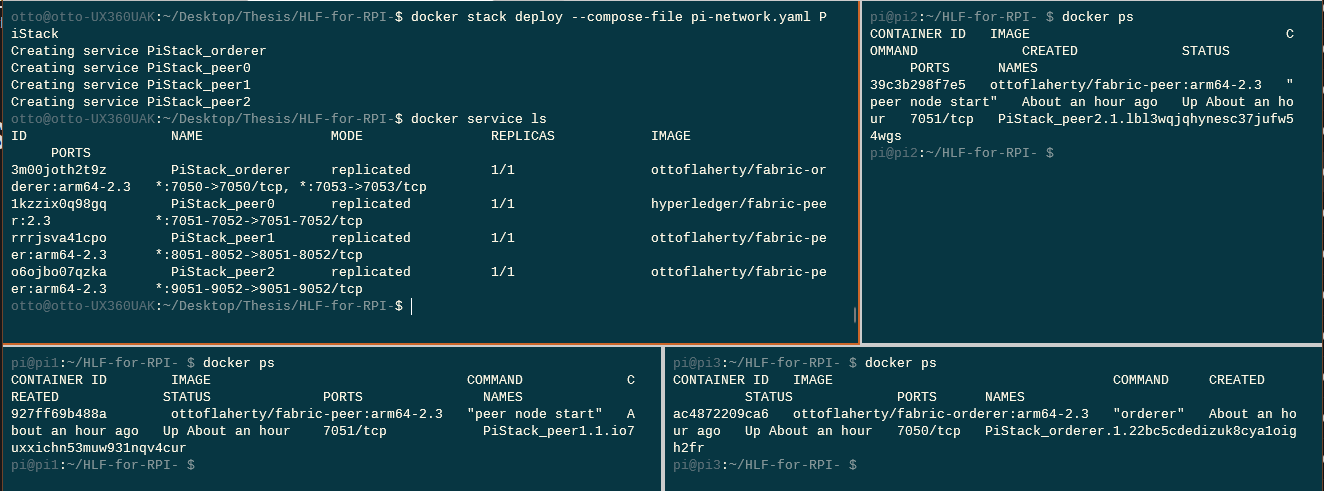
\includegraphics[width=1.2\columnwidth]{images/stackdeply.PNG}
    \caption{Using Stack Deploy to start up the network and seeing the containers run in the Pi's}
    \label{fig:my_label}
\end{figure}



\subsection{Creating a Channel}

As of Hyperledger Fabric version 2.3  creating a channel is now done through the Orderering service using the osnadmin binary. This binary requires the the paths Orderer Admin certificates to be given to it, along with the genesis block and the IP address and port of the Orderer node. As the orderer is placed on the 3rd Pi, this IP address is 192.168.86.150 and as we want to access the orderer as an admin we use port 7053, as defined in the orderer environment variables.

A shell script called setvars.sh has been created to export environmental variables into the terminal, and giving it the admin command will set the paths to the orderer admin certificates. This script must be called with source to enable these environment variables to be used in other commands like osnadmin.
\begin{verbatim}
    
$ osnadmin channel join --channel-id pichannel --config-block \ 
    ./channel-artifacts/pichannel.block -o 192.168.86.150:7053 \ 
    --ca-file "$ORDERER_CA" --client-cert "$ORDERER_ADMIN_TLS_SIGN_CERT" \ 
    --client-key "$ORDERER_ADMIN_TLS_PRIVATE_KEY"
\end{verbatim}

\begin{figure}
    \centering
    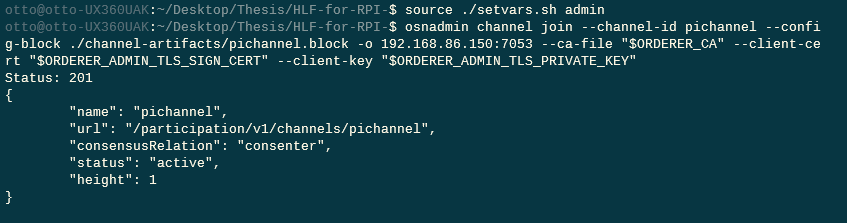
\includegraphics{osnadmin.PNG}
    \caption{Using the osnadmin binary to create the network}
    \label{fig:my_label}
\end{figure}



\subsection{Joining the Channel}
Once a network is created, the Peer nodes must be joined to it using the peer binary. The peer binary requires certain environment variables to be set aswell, even though they are not used in the binaries arguments. It requires the CORE\_PEER\_LOCALMSPID, CORE\_PEER\_TLS\_ROOTCERT\_FILE, CORE\_PEER\_MSPCONFIGPATH, CORE\_PEER\_ADDRESS and  FABRIC\_CFG\_PATH. The  FABRIC\_CFG\_PATH must be the path to a core.yaml file, this core.yaml file does not need to have the correct values set within it, but none the less the peer binary requires it, which is strange, but that is how the binary works. The CORE\_PEER\_ADDRESS and CORE\_PEER\_TLS\_ROOT\_CERTFILE must both be specifc to the peer that we are trying to acces, while the CORE\_PEER\_MSPCONFIGPATH and CORE\_PEER\_LOCALMSPID are just organisation specific and do not need to change when joining different peers. It is used as follows:

\begin{verbatim}
    source setvars.sh pi0
    peer channel join -b ./channel-artifacts/pichannel.block 
    peer channel getinfo -c pichannel
\end{verbatim}

These commands must be repeated for the two other peers:

\begin{verbatim}
    source setvars.sh pi1
    peer channel join -b ./channel-artifacts/pichannel.block 
    peer channel getinfo -c pichannel
\end{verbatim}

\begin{verbatim}
    source setvars.sh pi2
    peer channel join -b ./channel-artifacts/pichannel.block 
    peer channel getinfo -c pichannel
\end{verbatim}

\begin{figure}[h]
    \centering
    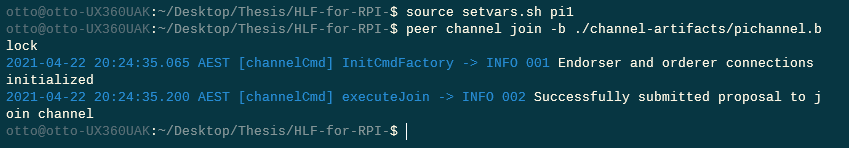
\includegraphics{pi1join.PNG}
    \caption{Joining the first peer to the network}
    \label{fig:my_label}
\end{figure}


\section{Using the Network}

Once all the peers are joined, the network is up and running. From this point a user could then go and add their own chaincodes and start running the network. Here we will detail this process and further describe how the network can be monitored.

\subsection{Adding Chaincode to the Network}

In this section we use chaincode provided by the Hyperledger Fabric Samples Github repository, as this thesis is not focused on the creation of chaincode, but of setting up a multiple machine Hyperledger Fabric network using low powered devices. The chaincode used from the Fabric Samples is the asset-transfer-basic chaincode.

\subsubsection{Packaging Chaincode}

The first step of setting up chaincode for a network is packaging it. This makes use of the peer binary, using its lifecycle chaincode package command. This command needs the path to the chaincode, the language of the chaincode and a label for the chaincode, from which it creates a tar file of the chaincode which can then be installed. This step only needs to be completed on one of the devices and has been tested from both the Raspberry Pi's and the laptop. When packaging Go chaincode some Go specific module must also be set as shown in the below code. We also set quite a few environment variables for this step, which can be set with the setvars.sh command giving it 'chaincode' as its argument.

\begin{verbatim}
    $ source setvars.sh chaincode
    $ pushd $CC_SRC_PATH
    $ GO111MODULE=on go mod vendor
    $ pop
    $ peer lifecycle chaincode package ${CC_NAME}.tar.gz --path \
      {CC_SRC_PATH} --lang ${CC_RUNTIME_LANGUAGE} --label ${CC_NAME}_${CC_VERSION}
\end{verbatim}

\begin{figure}[h]
    \centering
    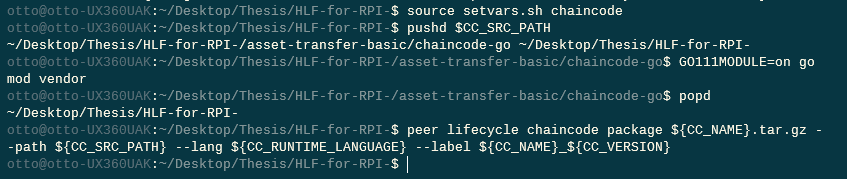
\includegraphics[width=1.2\columnwidth]{package chaincode.PNG}
    \caption{Setting go modules and packaging Chaincode}
    \label{fig:my_label}
\end{figure}

\subsubsection{Installing Chaincode}
Once chaincode has been packaged, it must then be installed on all peers in the network. This makes use of the peer binary, using its lifecycle chaincode install mode. This command also requires setting of the same environment variables as when joining peers to the network.

\begin{verbatim}
    $ source setvars.sh laptop
    $ peer lifecycle chaincode install ${CC_NAME}.tar.gz
    $ peer lifecycle chaincode queryinstalled
\end{verbatim}

This step must be done for all peers on the network, all of this can be done from the one device as the peer binary will use the addresses to find the Hyperledger Fabric containers on other devices. The output of query installed is saved to a log.txt file and then searched through to get the package ID which is used in a later step.

\begin{verbatim}
    $ source setvars.sh pi1
    $ peer lifecycle chaincode install ${CC_NAME}.tar.gz
    $ peer lifecycle chaincode queryinstalled
\end{verbatim}

\begin{verbatim}
    $ source setvars.sh pi2
    $ peer lifecycle chaincode install ${CC_NAME}.tar.gz
    $ peer lifecycle chaincode queryinstalled >&log.txt
    $ PACKAGE_ID=$(sed -n "/${CC_NAME}_${CC_VERSION}/
       {s/^Package ID: //; s/, Label:.*$//; p;}" log.txt)
\end{verbatim}


\begin{figure}[h]
    \centering
    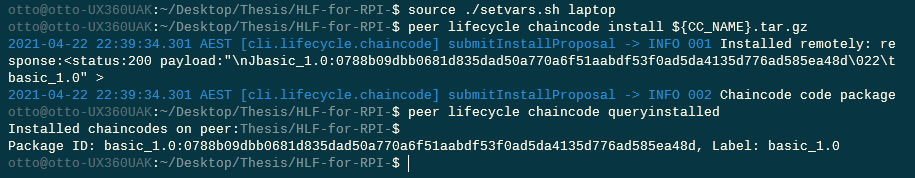
\includegraphics{install chaincode.PNG}
    \caption{Installing Chaincode on the Laptop}
    \label{fig:my_label}
\end{figure}


\subsubsection{Approving for Organisation}

Before chaincode can be commited to a channel, it must be first approved. In Hyperleger Fabric, approving a chaincode requires organisations to send an approval to the Orderering Service. Dependant on the policies set in the channel this may require all organisations, a majority of organisations or just a single organisation to send this message. In this network the policy to set a chaincode requires a majority approval from all organisations and as there is only one organisation in the channel, this is only necessary to do once. The approval is done through the peer lifecycle chaincode approveformyorg command, this command requires the orderes address, its certificates and various other arguments like the chaincode name, the full command is shown below.


\begin{verbatim}
    $ peer lifecycle chaincode approveformyorg -o $ORD_ADDR \
    --ordererTLSHostnameOverride orderer.example.com --tls \
    --cafile "$ORDERER_CA" --channelID $CHANNEL_NAME --name ${CC_NAME} \
    --version ${CC_VERSION} --package-id ${PACKAGE_ID} \
    --sequence ${CC_SEQUENCE} ${INIT_REQUIRED} ${CC_END_POLICY} ${CC_COLL_CONFIG}
\end{verbatim}
\begin{figure}[h]
    \centering
    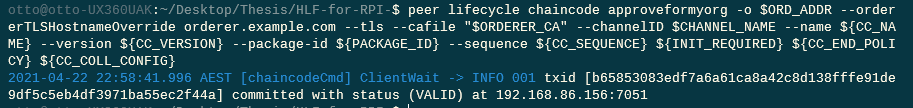
\includegraphics{images/approveformyorg.PNG}
    \caption{Approving a chaincode definition for an organisation}
    \label{fig:my_label}
\end{figure}

\subsubsection{Check Commitness Ready}

As an approval requires a user from each organisation to manually approve chaincode, it is useful to check which organisations in the network have already approved the chaincode and if it is ready to be commited to the channel. This is done through the peer lifecycle chaincode checkcommitreadiness command, which is used as follows.

\begin{verbatim}
    $ peer lifecycle chaincode checkcommitreadiness --channelID \
    $CHANNEL_NAME --name ${CC_NAME} --version ${CC_VERSION} \
    --sequence ${CC_SEQUENCE} ${INIT_REQUIRED} ${CC_END_POLICY} \
    ${CC_COLL_CONFIG} --output json 
\end{verbatim}

\begin{figure}[h]
    \centering
    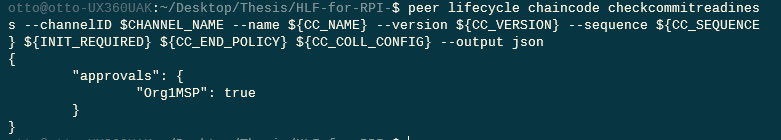
\includegraphics{images/checkcommitready.PNG}
    \caption{Checking the commit readiness of a chaincode on a channel}
    \label{fig:my_label}
\end{figure}

\subsubsection{Commiting Chaincode}

Once the chaincode is approved by the required members of the channel it can be commited to the channel, allowing users to create transactions on the network. This is done with the peer lifecycle chaincode commit command. This command requires the orderer address and certificates, the addresses and TLS certificates of all peers the chaincode has been installed on and other chaincode specific arguments.


\begin{verbatim}
    $ peer lifecycle chaincode commit -o $ORD_ADDR \
    --ordererTLSHostnameOverride orderer.example.com  \
    --tls --cafile "$ORDERER_CA" -C $CHANNEL_NAME --name \
    ${CC_NAME} --peerAddresses $PEER0_ADDR  --peerAddresses \  
    $PEER1_ADDR --peerAddresses $PEER2_ADDR --tlsRootCertFiles \ 
    $PEER0_ROOT_Cert --tlsRootCertFiles $PEER1_ROOT_Cert \ 
    --tlsRootCertFiles $PEER2_ROOT_Cert --version ${CC_VERSION} \ 
    --sequence ${CC_SEQUENCE} ${INIT_REQUIRED} \ 
    ${CC_END_POLICY} ${CC_COLL_CONFIG}
\end{verbatim}


\begin{figure}
    \centering
    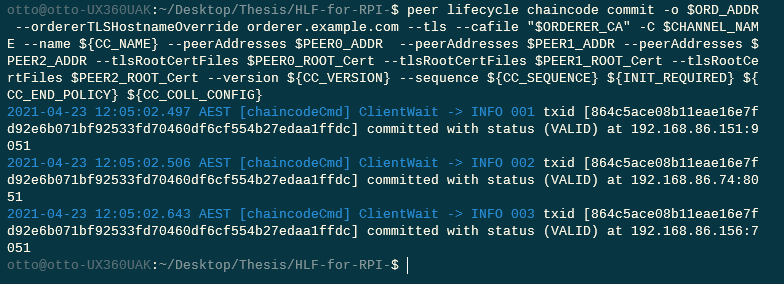
\includegraphics{images/chaincodecommit.PNG}
    \caption{Commiting Chaincode}
    \label{fig:my_label}
\end{figure}

\begin{figure}
    \centering
    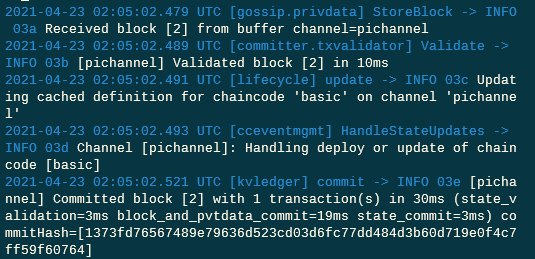
\includegraphics{images/peervalidatingcommit.PNG}
    \caption{Docker logs of a Peer node validating a chaincode commit}
    \label{fig:my_label}
\end{figure}

\subsection{Using Chaincode}


\section{Monitoring the Network}

Prometheus stuff
